\chapter{基于FPGA的循环神经网络加速器实验分析}
上一章详细介绍了循环循环神经网络加速系统的设计,包括系统总体架构设计,功能划分,软硬件设计及其具体实现,系统的各个组成部分分工协同,
并最终完成了系统的搭建。本章将从实验的角度对系统设计的各项目标进行检测,实验的内容包括验证系统的基本功能是否正常,系统的资源消耗是否合理,
以及系统的运行速度和功耗能否满足系统设计要求。最后,在完成上述实验的基础上,本章将对系统的优势进一步说明。
\section{实验方案设计}
\subsection{实验环境}
硬件平台:如图\ref{fig_board},本章实验采用Nexys4 DDR开发板作为本文系统的硬件平台。Nexys4 DDR开发板内部集成了Artix-7系列的FPGA芯片,型号为XCA100T-1CSG324C。
该芯片采用28nm的高效能/低功耗(HPL)制程技术,能够在极低功耗的前提下突破许多性能极限,广泛应用于低功耗的场景。此外,开发板还配置了容量为128MB的DDR存储器,
能满足多数应用的存储需求,Microblaze软处理器等技术支持也使得设计人员可以基于FPGA快速搭建SOC系统。低功耗,高能效,便捷性是本文选取Nexys4 DDR作为硬件平台的
重要原因,同时由于A7系列FPGA芯片的资源相对有限,而一般情况下,循环神经网络加速器需要消耗大量的资源,因此解决这一组矛盾也符合本文系统设计的初衷。

开发工具:本文使用Xilinx公司的FPGA开发套件,包括Vitis HLS, Vivado以及Vitis SDK。这些开发工具能提供从软件设计,硬件实现到软硬件系统的集成等系统
设计的全部任务流程。

神经网络训练:循环神经网络结构的搭建采用TensorFlow (Tensorflow Addons, TFA) 框架下的ESN网络模型,网络的训练方法是线性回归,该方法具有计算快,收敛性强等优势。
在完成网络参数的训练后需要将参数提取出来以进行后续的压缩过程。压缩算法的验证基于NumPy设计实现,简化网络的功能验证也在此环境下进行。最后保存训练好的
原始网络模型参数以及必要的压缩算法所需的数据。
\begin{figure}
	\centering
	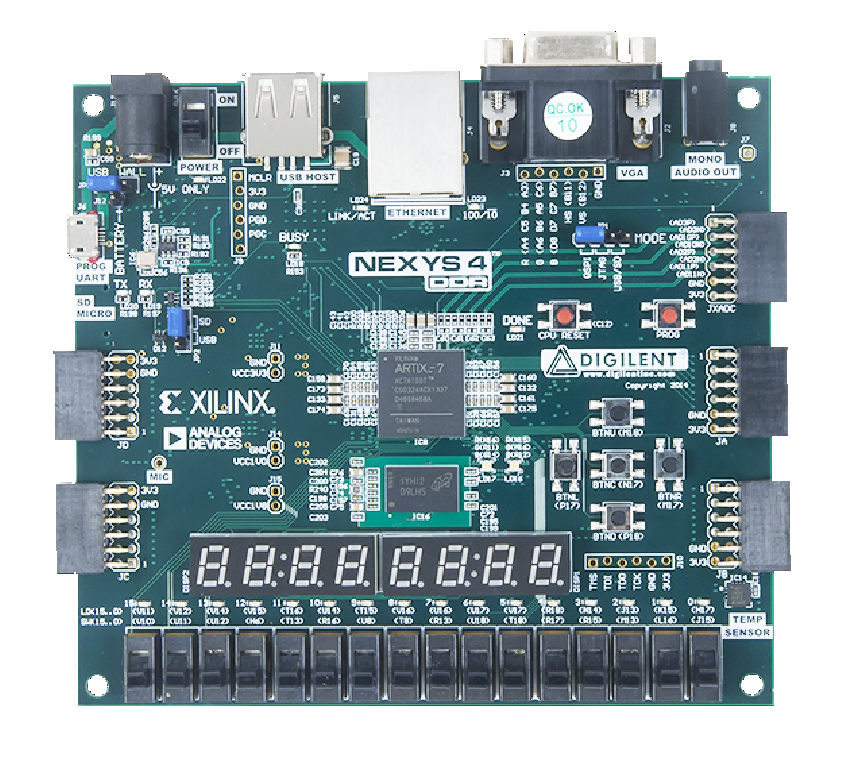
\includegraphics[width=0.6\columnwidth]{FPGA_board.eps}
	\caption{FPGA Nexys 4 DDR 开发版}
	\label{fig_board}
\end{figure}
\subsection{实验内容}
在算法分析及系统架构设计章节,本文详细的论述了系统设计的细节并展示了其所具有的潜在优势,例如从功能的角度,本文的系统设计能满足应用场景对
性能的弹性需求,能在资源有限的设备上独立运行,能实现和环境的数据交互等。从硬件实现的角度,本文所设计的硬件加速器具有高度复用的模块,极大的降低了
硬件资源的消耗。针对以上优势,本章设计了以下实验内容进行证明:

1.系统运行效果的实验:根据任务的难易程度以及任务的输入输出特点,本文选取了不同的测试集进行系统功能的测试。测试集包括单输入单输出系统:
NARMA10,NARMA30和复杂二阶问题,多输入单输出系统:耶拿天气预报数据集,多输入多输出系统:两入两出非线性系统。系统在运行这些任务时需要测试的功能
包括更改简化网络的模型尺寸,状态采样以及原始网络模型的压缩等。系统功能的正常是系统设计的首要目标,也是系统功能优势的实际体现。

2.加速器性能实验:本文对循环神经网络前向传播过程设计了专用硬件架构以实现加速的目的,加速器性能的主要指标有资源消耗,数据吞吐量(速度)以及功耗。
本实验将对这些指标分别进行测量,并将其与硬件设计相联系,说明本文加速器设计的特点和优势。

\subsection{系统运行效果}
实验设定:系统运行不同的任务,在连续输入的过程中切换模型尺寸,并以该尺寸的简化网络模型进行前向传播。简化网络模型的权重参数的生成有两种方法:
基于状态采样的模型生成方法和基于预置投影矩阵的模型生成方法,这两种方法分别对应系统的两种应用环境:异常状态环境和普通环境。在普通环境下,
网络的实际状态与预存的状态空间偏离较小,通过增大投影空间的方法可以实现状态的“准确”近似;在异常状态环境下,由于特征空间是有限的,无法囊括
所有的状态,少量实际存在的状态将在压缩的过程中被合理的丢失,然而在系统实际运行过程中难免会遇到这种情况,因此系统需要和实际环境进行数据交换,
通过采样的方法生成网络的权重参数。

本实验测量两种压缩模型生成方法下的模型预测效果。连续输入的序列长度为1000个,在完成该段序列的预测后,系统将会切换简化网络的模型尺寸并进行下一段序列的预测。
本实验依次设定简化网络模型阶数为10,20,30,40,60,80。实际上,在硬件支持的简化模型最大尺寸以下,简化网络模型尺寸可以设定为任意整数值。
%说明压缩算法能在边缘设备实现,加速器可以运行不同尺寸的网络模型。

\subsubsection{复杂二阶问题}
复杂二阶问题建模了一个二阶动态系统,该系统的数据依赖呈现指数相关的关系,即输入序列中的关键信息会被指数放大,而无关特征则会被迅速遗忘。
其数学表达为
\begin{equation}
	y(t+1) = \frac{y(t)y(t-1)(y(t)+0.25)}{1+y^2(t)+y^2(t-1)} + u(t)
\end{equation}
其中\(u(t)\)是在区间\([0,0.5]\)上生成的均匀分布的随机数。
\begin{center}
\begin{table}
	\caption{在二阶问题上简化网络不同模型尺寸的预测精度}
	\renewcommand\arraystretch{1.2}
	\setlength{\tabcolsep}{12pt}
	\begin{tabular}{ccccccc}
	\toprule
		 							&	10		&	20		&	30		&	40		&	60		&	80		\\	\midrule
	Sample M.\(\times 10^{-4}\)	&	2.99	&	2.58	&	2.46	&	0.81	&	0.25	&	0.11	 \\	\hline
	PreStore M.\(\times 10^{-4}\)&	36.3	&	18.5	&	9.9		&	6.9		&	1.7		&	0.53	\\	
	\bottomrule
	\label{tab:second}
	\end{tabular}
\end{table}
\vspace{-3em}
\end{center}



系统在二阶问题任务上的运行效果如图\ref{fig:second}所示,可以看出不同尺寸的简化网络模型的预测值均能较好的还原系统的真实输出。这里系统的真实输出可以
用原始网络模型的预测值进行准确的代替,一方面是因为原始网络模型的输出和系统真实输出误差较小,另一方面是因为在实际情况下测量系统的真实输出一般具有
滞后性,并且可能存在测量成本大等无法获得真实数据等情况。图中左侧是基于采样方法生成的简化网络模型,由上至下,模型的阶数依次增加。其中10阶的简化网络模型
预测效果和系统真实输出存在明显的偏差,随着简化网络模型尺寸的增大,模型的预测逐渐贴合系统的真实输出。图中右侧为基于预置投影矩阵方法生成的简化网络模型,
图中显示,该方法生成的简化网络模型在不同的模型尺寸下均拥有较小的误差。这说明小尺寸网络模型依然能胜任二阶问题的模型预测,网络精度的调节可以在
小尺寸网络的基础上进行小幅度改变即可。

表\ref{tab:second}展示了两种模型生成方法下简化网络不同尺寸的预测精度,误差的数值随着模型尺寸的增加而降低,其中采样方法生成的简化网络误差
降低更加明显。这说明了状态空间中越大,状态信息越丰富,其所生成的投影空间和和真实的特征空间偏差越小。由于预置的投影矩阵的生成往往采样了
足够多的状态数据,因此即使在相同的模型尺寸下,通过预存投影矩阵的方法生成的模型预测精度高于现场采样生成模型的精度。但是这并不能说明采样
方法不是系统所需要的功能。相反,由于该方法不依赖于任何先验信息,可以和环境交互数据,这使得即使系统处在异常环境中,也具有较高的预测能力。
两种方法互为补充,共同实现系统高精度预测的功能。
\begin{figure}
	\centering
	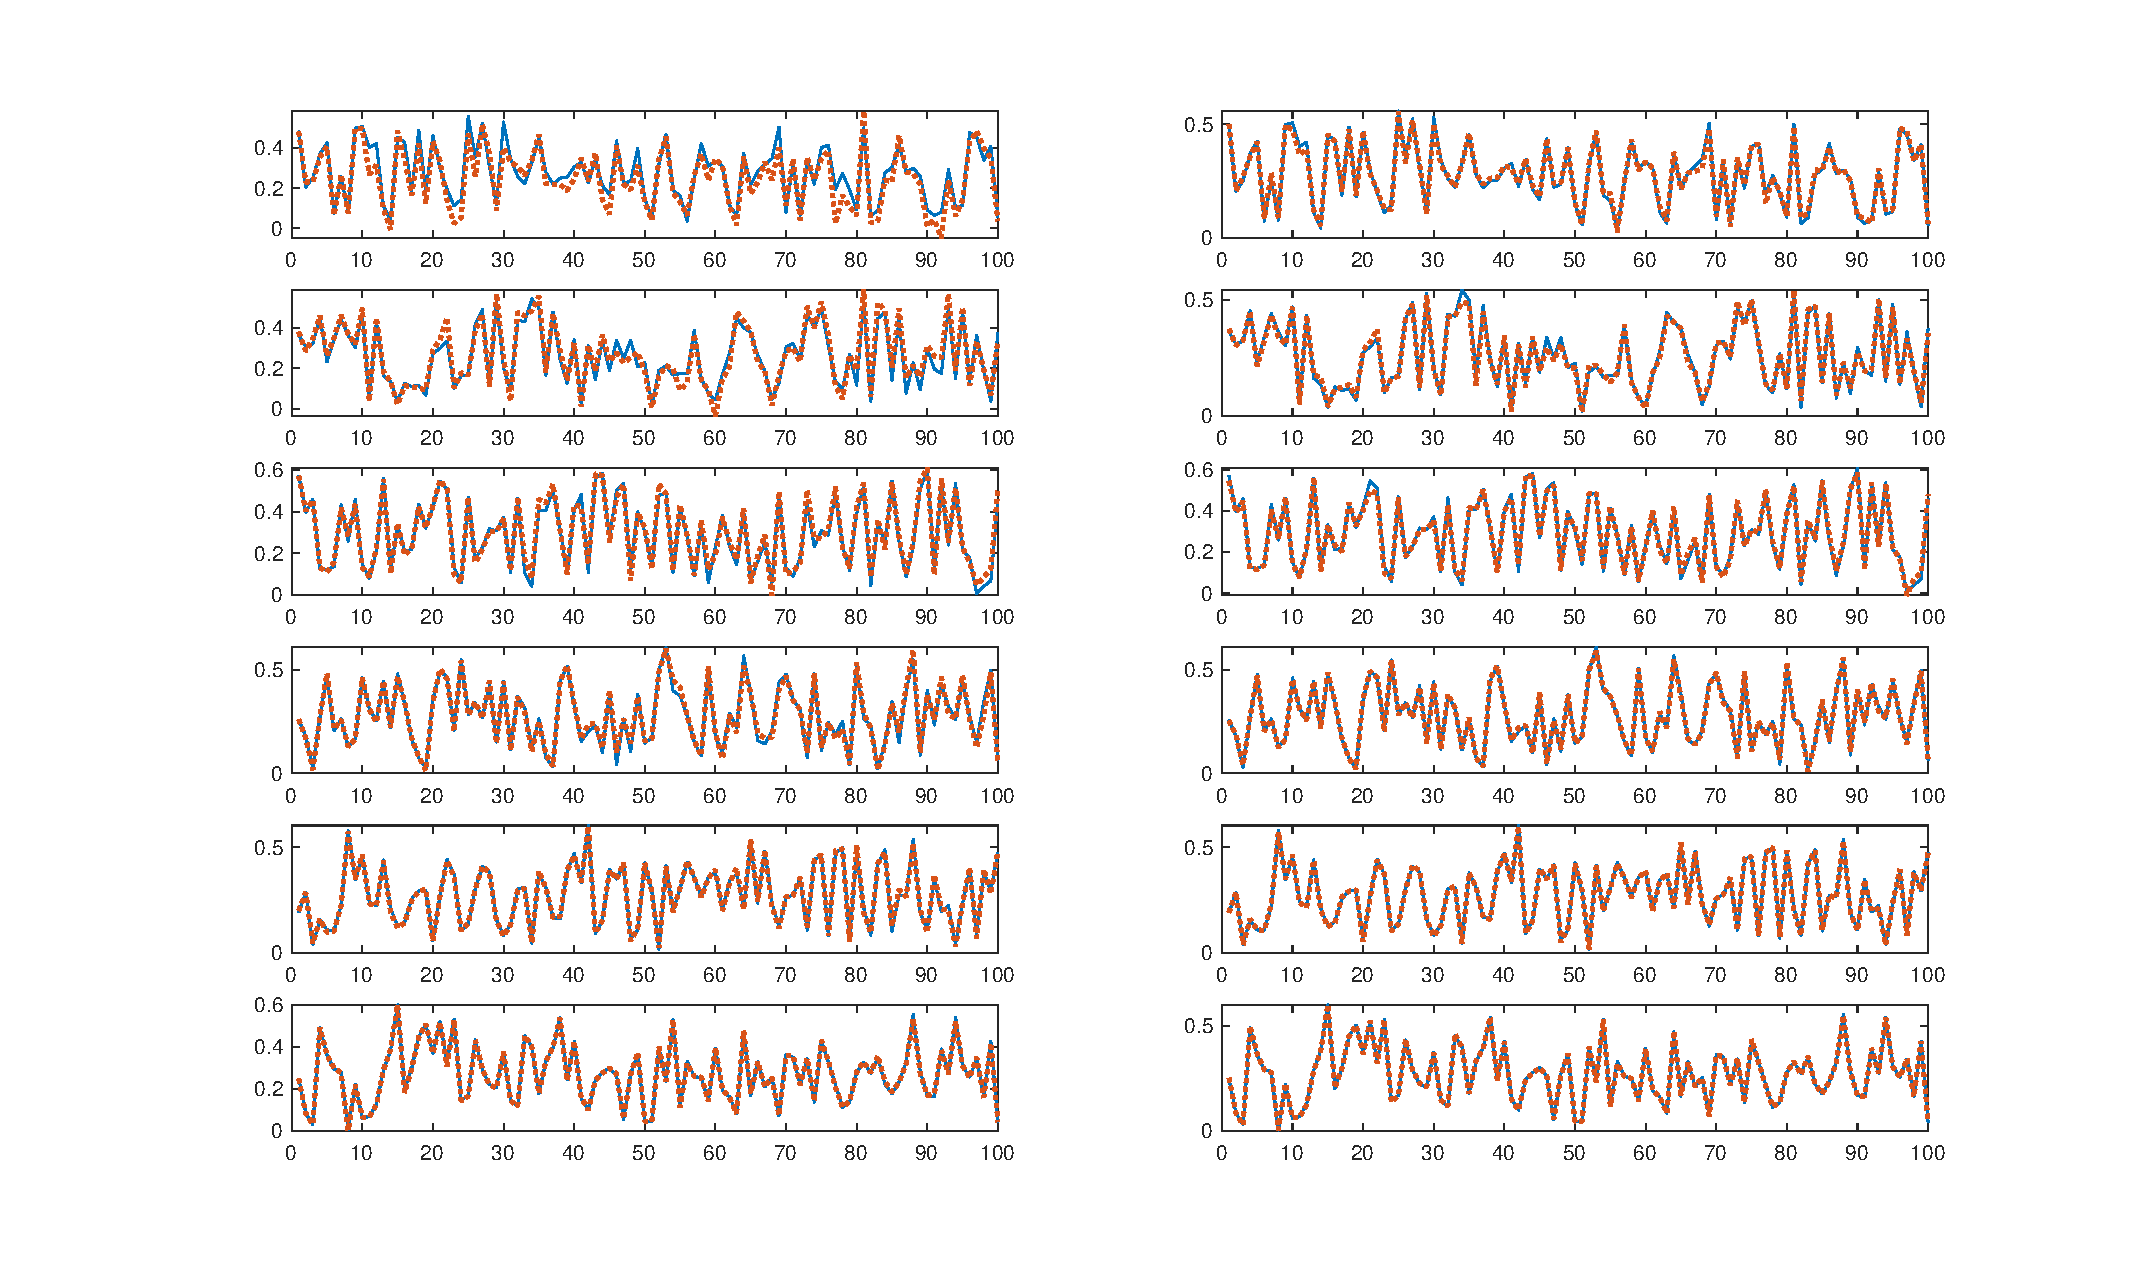
\includegraphics[width=1\columnwidth]{exp/fig_secondOrder.eps}
	\caption{在复杂二阶问题任务上的系统运行效果,图中左侧为使用采样方法生成简化网络,右侧为使用预存投影矩阵方法生成简化网络,图中自上至下表示的网络阶数分别
	为10,20,30,40,60,80。实线表示原始网络的模型预测值,虚线表示简化网络的模型预测值。}
	\label{fig:second}
\end{figure}

本文所设计的系统在二阶问题的任务的解决上,系统能够发现应用的实现难度较低进而主动降低简化网络模型的尺寸,并以较小的模型尺寸进行前向传播,
实现了高速的模型预测。相较于其他神经网络加速方法的一次性设计,本文的系统对应用的难易具有一定的感知能力。

\subsubsection{两个NAMA系统}
NARMA(Nonlinear Auto Regressive Moving Average)定义了具有长期依赖关系的动态系统,即很久以前的输入对系统当前的输出仍存在影响。循环神经
网络尽管能够学习这些长程依赖关系,但是依然存在一些难以解决的问题,例如对处理此类任务的循环神经网络进行压缩。压缩过程中损失的信息可能导致
网络失去长期记忆进而功能瘫痪。本文选取该应用进行系统运行效果测试,以验证系统在复杂应用中是否依然具有适用性。NARMA10系统的数学表达为
\begin{equation}
	y(t) = 0.3y(t-1) + 0.05y(t-1)\sum_{i=1}^{10}y(t-i) + 1.5u(t-9)u(t) + 0.1
\end{equation}
NARMA30系统的数学表达为
\begin{equation}
	y(t) = 0.2y(t-1) + 0.04y(t-1)\sum_{i=1}^{30}y(t-i) + 1.5u(t-29)u(t) + 0.001
\end{equation}


\begin{figure}
	\centering
	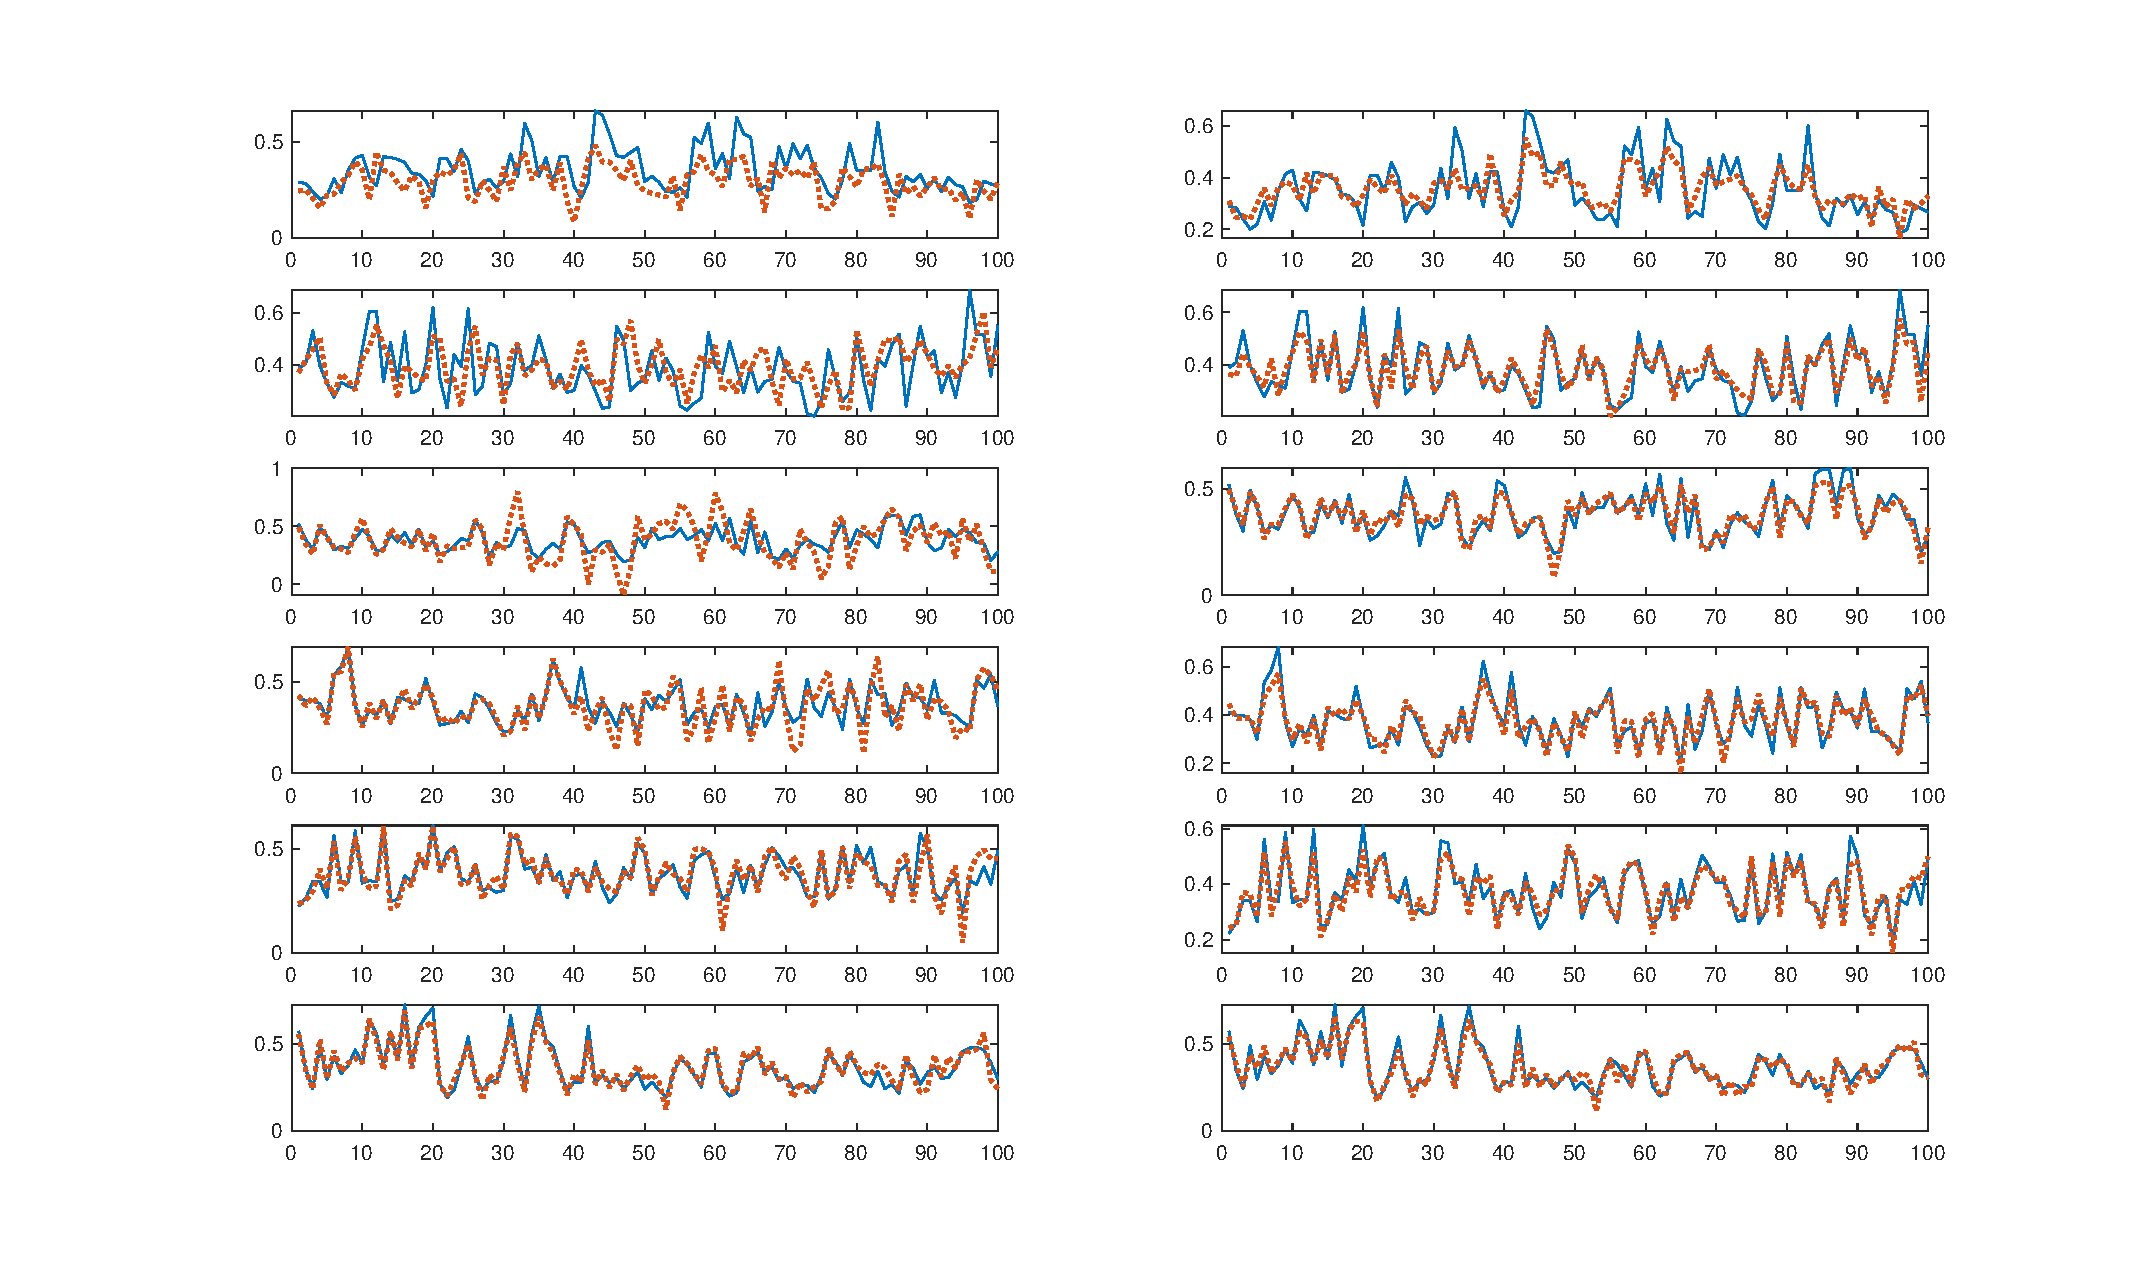
\includegraphics[width=1\columnwidth]{exp/fig_narma10.eps}
	\caption{在NARMA10任务上的系统运行效果,图中左侧为使用采样方法生成简化网络,右侧为使用预存投影矩阵方法生成简化网络,图中自上至下表示的网络阶数分别
	为10,20,30,40,60,80。实线表示原始网络的模型预测值,虚线表示简化网络的模型预测值。}
	\label{fig:second}
\end{figure}

\begin{figure}
	\centering
	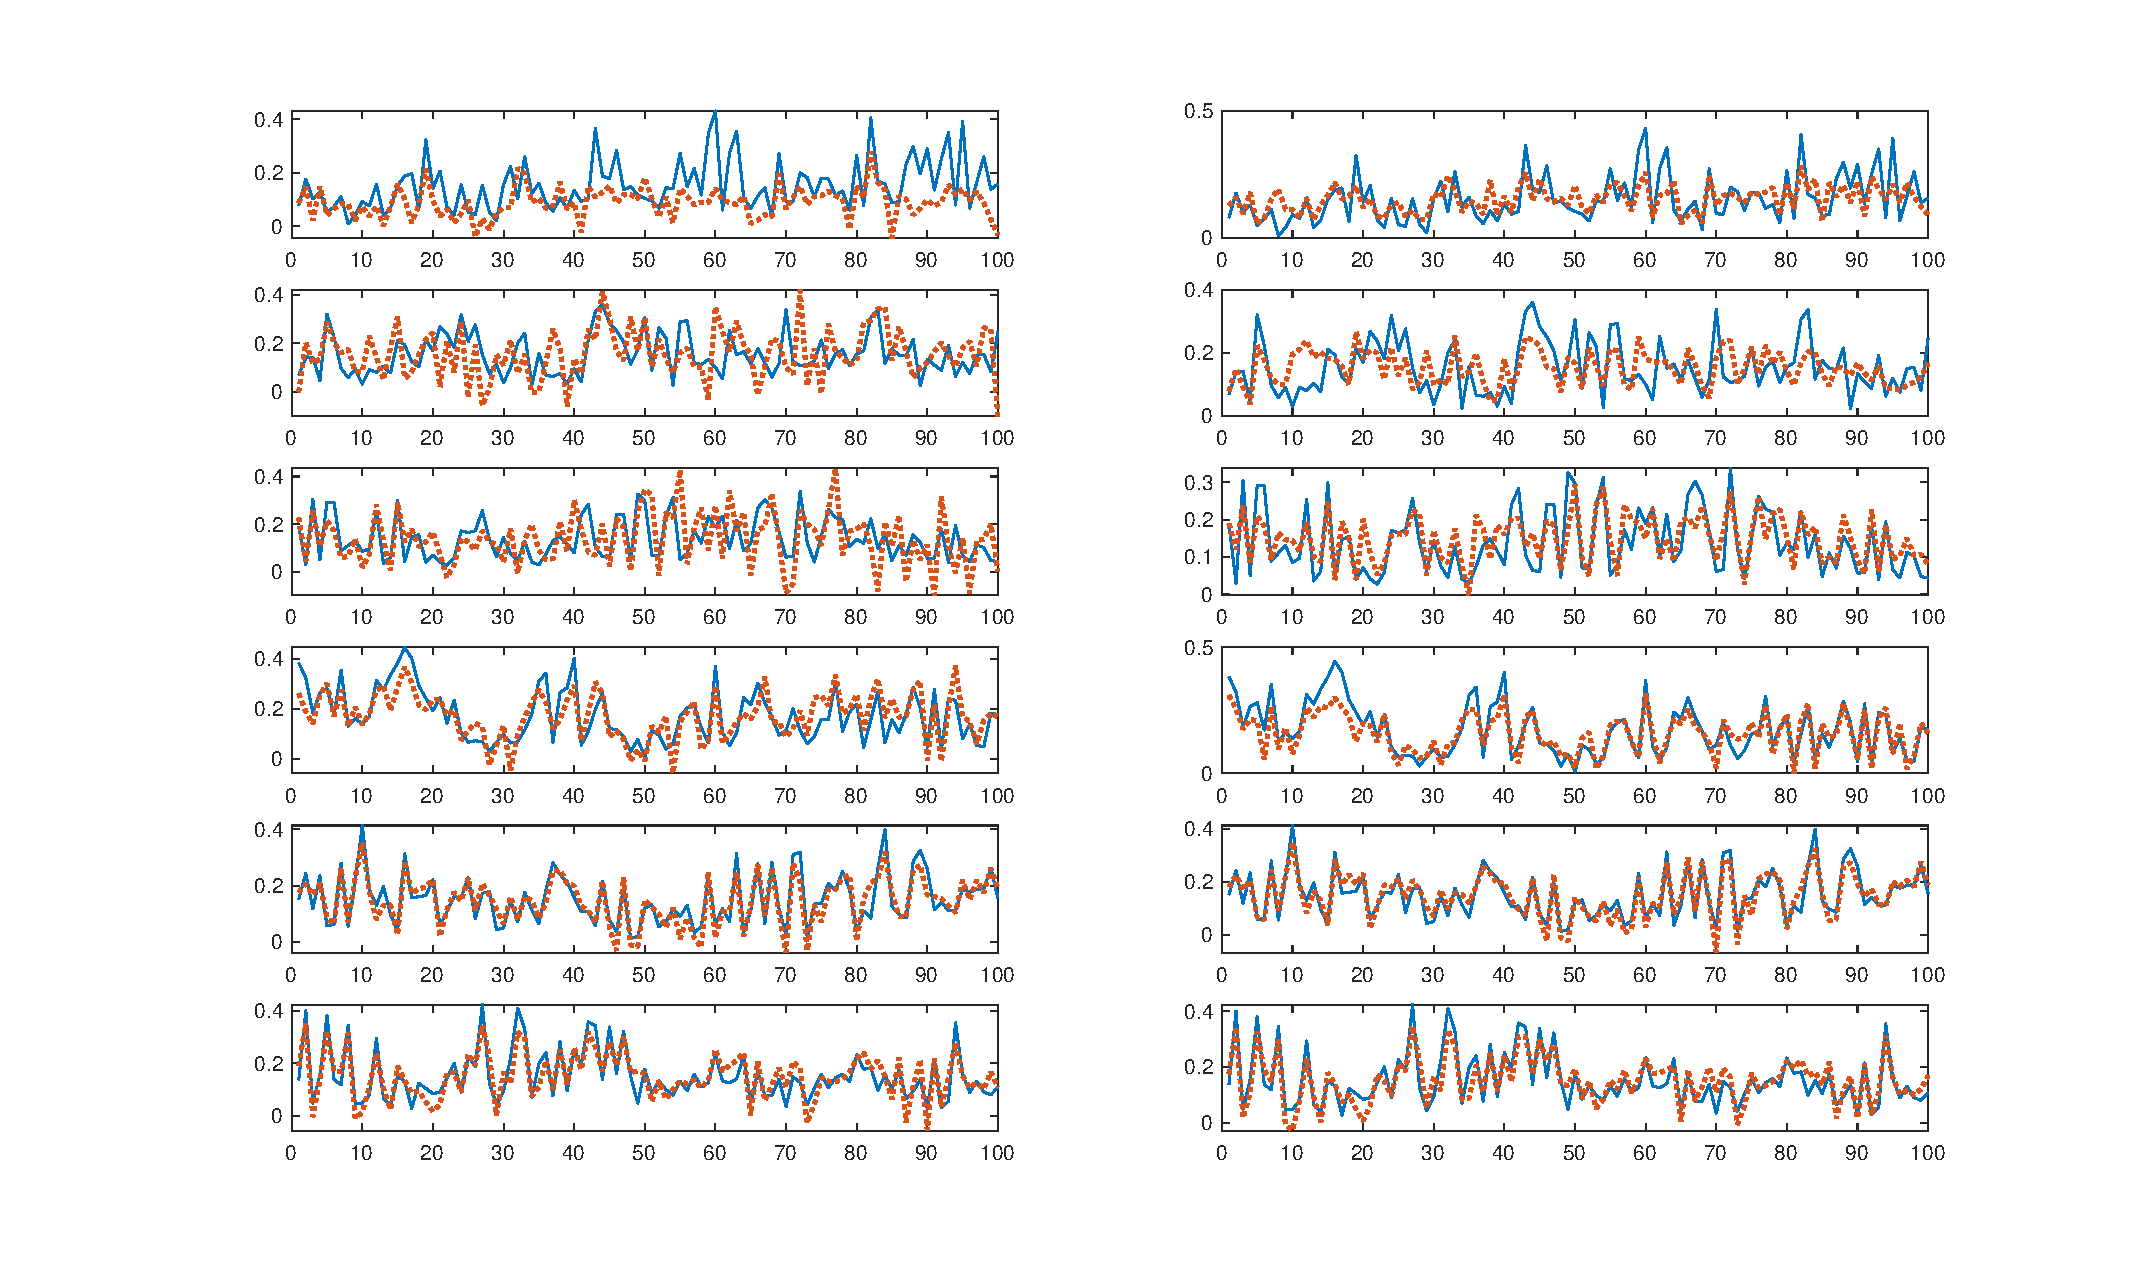
\includegraphics[width=1\columnwidth]{exp/fig_narma30.eps}
	\caption{在NARMA30任务上的系统运行效果,图中左侧为使用采样方法生成简化网络,右侧为使用预存投影矩阵方法生成简化网络,图中自上至下表示的网络阶数分别
	为10,20,30,40,60,80。实线表示原始网络的模型预测值,虚线表示简化网络的模型预测值。}
	\label{fig:second}
\end{figure}


采样方法 样本覆盖的位置精度高
在该类应用中的优势

最后对系统运行效果进行总结
%\subsubsection{多入多出系统}
%\begin{figure}
%	\centering
%	\includegraphics[width=1\columnwidth]{exp/fig_2In2Out.eps}
%	\caption{在两输入两输出系统任务上的系统运行效果,图中左侧为使用采样方法生成简化网络,右侧为使用预存投影矩阵方法生成简化网络,图中自上至下表示的网络阶数分别
%	为10,20,30,40,60,80。实线表示原始网络的模型预测值,虚线表示简化网络的模型预测值。}
%	\label{fig:second}
%\end{figure}
%
%
%\subsubsection{耶拿气候集}
%
%\begin{figure}
%	\centering
%	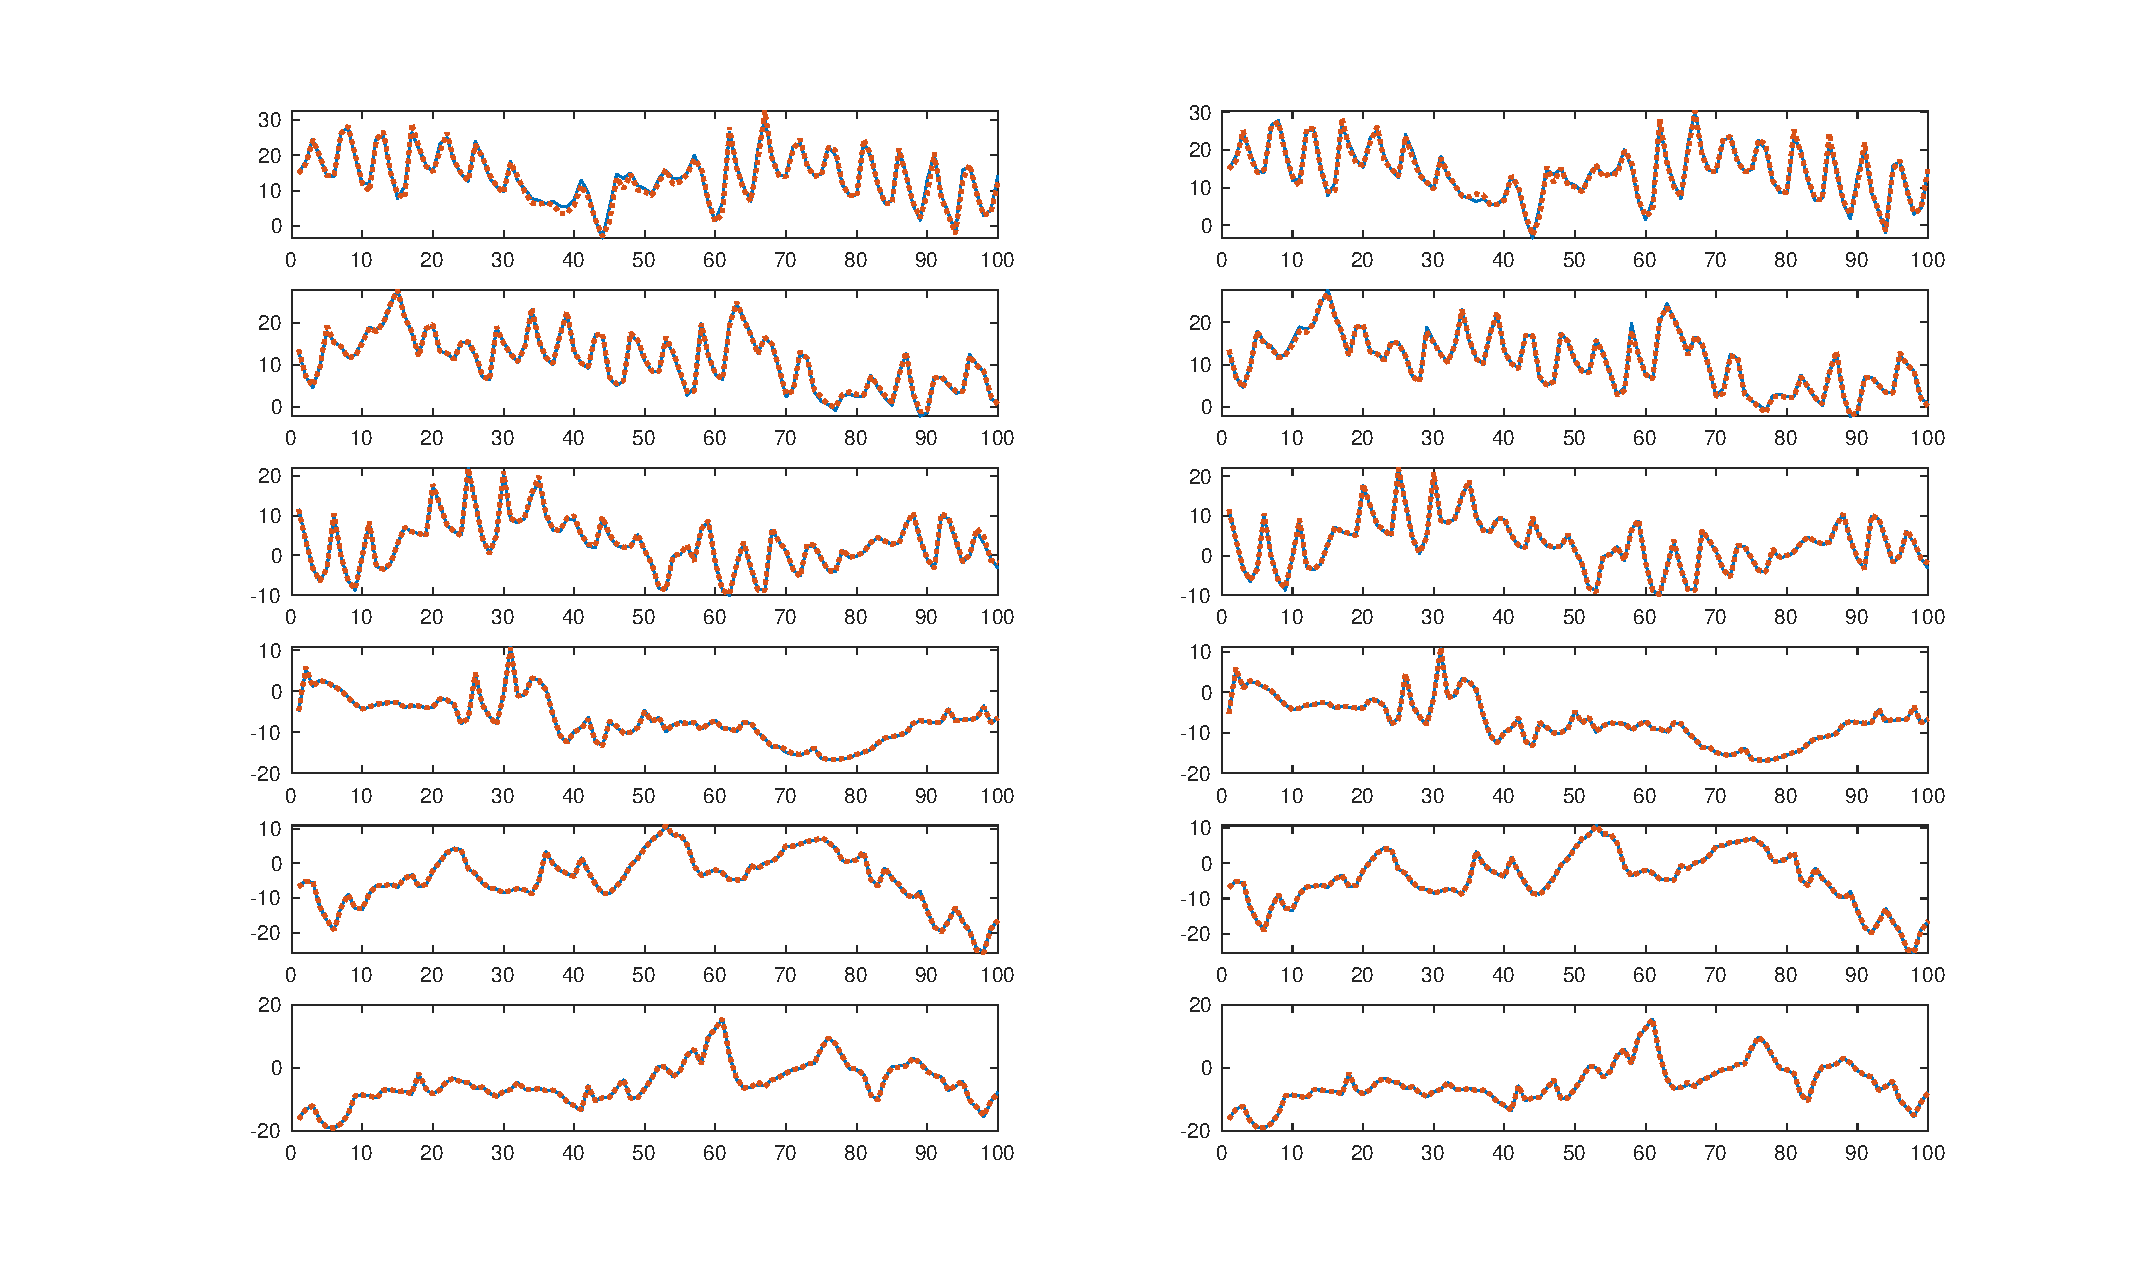
\includegraphics[width=1\columnwidth]{exp/fig_weather.eps}
%	\caption{在耶拿气候预测任务上的系统运行效果,图中左侧为使用采样方法生成简化网络,右侧为使用预存投影矩阵方法生成简化网络,图中自上至下表示的网络阶数分别
%	为10,20,30,40,60,80。实线表示原始网络的模型预测值,虚线表示简化网络的模型预测值。}
%	\label{fig:second}
%\end{figure}
